%% 
%% Copyright 2019-2021 Elsevier Ltd
%% 
%% This file is part of the 'CAS Bundle'.
%% --------------------------------------
%% 
%% It may be distributed under the conditions of the LaTeX Project Public
%% License, either version 1.2 of this license or (at your option) any
%% later version.  The latest version of this license is in
%%    http://www.latex-project.org/lppl.txt
%% and version 1.2 or later is part of all distributions of LaTeX
%% version 1999/12/01 or later.
%% 
%% The list of all files belonging to the 'CAS Bundle' is
%% given in the file `manifest.txt'.
%% 
%% Template article for cas-sc documentclass for 
%% single column output.

\documentclass[a4paper,fleqn]{cas-dc}

% If the frontmatter runs over more than one page
% use the longmktitle option.

%\documentclass[a4paper,fleqn,longmktitle]{cas-sc}

\usepackage[numbers]{natbib}
\usepackage{acro}

\DeclareAcronym{2d}{
	short=2D,
	long=two-dimensional,
}
\DeclareAcronym{3d}{
	short=3D,
	long=three-dimensional,
}
\DeclareAcronym{a0}{
	short=A$_0$,
	long=antisymmetric fundamental Lamb wave mode,
}
\DeclareAcronym{ccd}{
	short=CCD,
	long=correlation coefficient deviation,
}
\DeclareAcronym{cfrp}{
	short=CFRP,
	long=carbon fiber reinforced polymer,
}
\DeclareAcronym{di}{
	short=DI,
	long=damage index,
}
\DeclareAcronym{dau}{
	short=DAU,
	long=data acquisition unit,
}
\DeclareAcronym{dof}{
	short=DOF,
	long=degree of freedom,
}
\DeclareAcronym{emi}{
	short=EMI,
	long=electromechanical impedance,
}
\DeclareAcronym{fem}{
	short=FEM,
	long=finite element method,
}
\DeclareAcronym{fbg}{
	short=FBG,
	long=fiber Bragg grating,
}
\DeclareAcronym{gw}{
	short=GW,
	long=guided waves,
}
\DeclareAcronym{gll}{
	short=GLL,
	long=Gauss-Lobatto-Legendre,
}
\DeclareAcronym{gpu}{
	short=GPU,
	long=graphics processing unit,
}
\DeclareAcronym{hsc}{
	short=HSC,
	long=honeycomb sandwich composite,
}
\DeclareAcronym{ncn}{
	short=NCN,
	long=National Science Centre,
}
\DeclareAcronym{madif}{
	short=MADIF,
	long=model assisted damage identification function,
}
\DeclareAcronym{mapd}{
	short=MAPD,
	long=mean absolute percentage deviation,
}
\DeclareAcronym{pnn}{
	short=PNN,
	long=probabilistic neural networks,
}
\DeclareAcronym{pzt}{
	short=PZT,
	long=piezoelectric transducer,
}
\DeclareAcronym{rms}{
	short=RMS,
	long=root mean square,
}
\DeclareAcronym{rmsd}{
	short=RMSD,
	long=root mean square deviation,
}
\DeclareAcronym{rve}{
	short=RVE,
	long=representative volume element,
}
\DeclareAcronym{s0}{
	short=S$_0$,
	long=symmetric fundamental Lamb wave mode,
}
\DeclareAcronym{sem}{
	short=SEM,
	long=spectral element method,
}
\DeclareAcronym{scs}{
	short=SCS,
	long=sandwich composite structure,
}
\DeclareAcronym{shm}{
	short=SHM,
	long=structural health monitoring,
}
\DeclareAcronym{sldv}{
	short=SLVD,
	long=scanning laser Doppler vibrometer,
}

\usepackage[ruled,vlined]{algorithm2e}
\usepackage{multirow}
\usepackage{amsthm}
\usepackage{multicol}
\usepackage{etoolbox,ragged2e,siunitx,mathtools}
\graphicspath{{Figures/}} 
%\usepackage[authoryear]{natbib}
%\usepackage[authoryear,longnamesfirst]{natbib}

%%%Author macros
\def\tsc#1{\csdef{#1}{\textsc{\lowercase{#1}}\xspace}}
\tsc{WGM}
\tsc{QE}
%%%

% Uncomment and use as if needed
%\newtheorem{theorem}{Theorem}
%\newtheorem{lemma}[theorem]{Lemma}
%\newdefinition{rmk}{Remark}
%\newproof{pf}{Proof}
%\newproof{pot}{Proof of Theorem \ref{thm}}

\begin{document}
\let\WriteBookmarks\relax
\def\floatpagepagefraction{1}
\def\textpagefraction{.001}

% Short title
\shorttitle{Model-assisted guided-wave based approach for debonding assessment in honeycomb sandwich structures}

% Short author
\shortauthors{P. Fiborek, P. Kudela}  

% Main title of the paper
\title [mode = title]{Model-assisted guided-wave based approach for debonding assessment in honeycomb sandwich structures}

% Title footnote mark
% eg: \tnotemark[1]
%\tnotemark[1] 

% Title footnote 1.
% eg: \tnotetext[1]{Title footnote text}
%\tnotetext[1]{<footnote text>} 

% First author
%
% Options: Use if required
% eg: \author[1,3]{Author Name}[type=editor,
%       style=chinese,
%       auid=000,
%       bioid=1,
%       prefix=Sir,
%       orcid=0000-0000-0000-0000,
%       facebook=<facebook id>,
%       twitter=<twitter id>,
%       linkedin=<linkedin id>,
%       gplus=<gplus id>]

\author[1]{Piotr Fiborek}[type=editor,
orcid=0000-0002-5030-3312]

% Corresponding author indication
\cormark[1]

% Footnote of the first author
%\fnmark[1]

% Email id of the first author
\ead{pfiborek@imp.gda.pl}

% URL of the first author
\ead[url]{www.imp.gda.pl}

% Credit authorship
% eg: \credit{Conceptualization of this study, Methodology, Software}
%\credit{<Credit authorship details>}

% Address/affiliation
\affiliation[1]{organization={Institute of Fluid Flow Machinery, Polish Academy of Sciences},
            addressline={Fishera 14 st.}, 
            city={Gdańsk},
%          citysep={}, % Uncomment if no comma needed between city and postcode
            postcode={80-231},
            country={Poland}}

\author[1]{Pawel Kudela}[orcid=0000-0002-5130-6443]

% For a title note without a number/mark
%\nonumnote{}

\begin{abstract}[S U M M A R Y]
	This study aims to assess the debonding of the carbon skin from the honeycomb core in the sandwich panel based on guided wave propagation.
	The effect of damage on wave propagation in the panel was determined using numerical simulations.
	The two most common honeycomb core models found in the literature are a homogenized, orthogonal continuous medium and a real geometry core modelled by finite elements, usually using commercial software.
	In a simplified model, the results are in good agreement only for low frequencies.
	In this paper, the panel wad modelled by the time-domain spectral element method taking into account the real geometry of the honeycomb core.
	The presented model was compared with the homogenized model of the 
	The result of the parametric study is a function of damage influence on the amplitude of propagating waves.
\end{abstract}
\begin{keywords}
Honeycomb, Debonding, Computational modelling, Spectral element methods, 
\end{keywords}

\maketitle

\section{Introduction}
\label{sec:intro}
\Ac{hsc} is a multi-layered structure composed of the mid-core with the geometry of honeycomb sandwiched between thin skins.
They are widely used in the aerospace, marine and automotive industries due to their high strength-to-weight ratio, high energy absorption capability and effective acoustic insulation.
However, these complex structures are exposed to various types of damage that are not found in metal alloy materials, e.g. hidden disbonds between the skin and the core, delamination of the skin plates, or the core impact damage.
The damage can occur during a manufacturing process, storage or in-service life; thus, advanced methods for online damage detection are required.

The Guided Wave (GW) based method is one of the structural health monitoring (SHM) techniques with very high potential for damage detection and localization in HSC \cite{mustapha2011assessment, sikdar2016guided, sikdar2016ultrasonic,radzienski2016assessment, yu2019core}.
Assessing the damage severity in structural materials requires a database of the damage influence on system response \cite{worden2007fundamental}.
In the case of \ac{hsc}, many factors affect the \ac{di} magnitude, such as damage localisation, material properties and dimensions, the sensor position relative to the core cell and the boundary conditions.
Determining \ac{di} by experimental means becomes very complicated, expensive and time-consuming, considering all the factors.
Therefore, numerical analysis and computer simulations become the only practical tool to achieve the goal.

The most common \ac{hsc} numerical model used in analysing \acp{gw} and \ac{emi} found in the literature is based on the \ac{fem}.
Although the numerical results are close to the experimental results, the models have some limitations in performing the simulations with reasonable computation time and operating memory consumption.
In order to alleviate these limitations, the following techniques are employed: (i) reduction of the sample dimensions \cite{hosseini2013numerical, tian2015wavenumber}, (ii) homogenisation of the core properties \cite{catapano2014multi, zhou2020debonding}, (iii) a simplified \acl{2d} model based on a cross-section of the panel~ \cite{li2019detection} and (iiii) omission of an adhesive layer \cite{mustapha2013non}.

The time and memory consumption of the \ac{fem} simulations is due to the high spatial resolution needed to converge the numerical results.
When first-order elements are used, up to 20 nodes per the shortest wavelength of interest is recommended by Moser et al. \cite{moser1999modeling}.
At a time when the operational capabilities of personal computers were severely limited, several methods derived from classic \ac{fem} were developed to increase the efficiency of calculations.
The \ac{bem} has been widely used for wave propagation in infinite or semi-infinite areas \cite{brebbia1984boundary}.
This method uses the fundamental solution of a \ac{pde} with the approximation only at the boundary of the domain.
The \ac{fdm} also has found application in elastic wave modelling \cite{delsantoO1992connection}.
The solution of the \ac{pde} is realised by the Taylor expansion with the arbitrary number of terms that determines the order of accuracy \cite{willberg2015simulation}.
The main disadvantage of this method is the loss of numerical stability for the structure with varying material properties.

To avoid this drawback, Delsanto et al. developed the \ac{lisa} with the combination of a sharp interface model to connect to different domains \cite{delsantoO1992connection}. This method is the extension of the \ac{fdm} in which iteration equations are obtained directly from heuristic consideration \cite{willberg2015simulation}.
The \ac{lisa} is highly numerically efficient because local interactions between elements are directly transferred for numerical calculations.

However, no usage of the \ac{bem}, \ac{fdm} and \ac{lisa} in \ac{hsc} modelling has been documented in the literature, supposedly due to the complex geometry of the core.
Realistic shape of the core can be implemented while keeping numerical efficiency using a technique based on high-order elements.
The implementations of this technique have been developed in recent years, achieving convergence even at six nodes in case of \ac{gw} propagating in isotropic plates \cite{willberg2012comparison}.
One of the implementations is a method based on Lagrange polynomials as a shape function and the \ac{gll} for integration scheme, termed the \ac{sem}.
The \ac{sem} was initially developed by Patera \cite{patera1984spectral} for the numerical solution of the fluid flow in a channel.
The method has also been successfully employed for acoustic wave propagation in geological structures \cite{seriani1994spectral, komatitsch2000simulation} and \ac{gw} propagation in engineering elements \cite{kudela2007wave, ostachowicz2011guided, rucka2010experimental,rekatsinas2017cubic}.
The \ac{sem} can be applied to complex structures, e.g. stiffened panels \cite{schulte2011simulation, lonkar2014modeling}.
The versatility of the method is also related to the use of hybrid elements in combination with \ac{fem} formulation \cite{ha2009optimizing} and non-linear issues \cite{yu2020time, li2021hybrid}.

Due to the fast convergence and flexibility of the \ac{sem}, Kudela \cite{kudela2016parallel} applied the method to the \ac{hsc} model with the \ac{fcgm}.
However, the author used \ac{3d} elements to model the core walls resulting in a huge number of \acp{dof}.
The model size could be reduced if the shell element replaced the solid one.
In addition, the surface-mounted \ac{pzt} is omitted in the above model, and a concentrated force is used as the disturbance source.
The sensor mesh would have to coincide with the plate mesh or use the coupling between both meshes to include the \acp{pzt} in the simulation.
Such coupling can be realised using an interface based on Lagrange multipliers proposed by Farhat and Roux for domain decomposition in \ac{fem} \cite{farhat1991method}.
Ashwin et al. implemented the interface for the \ac{sem} but did not adopt it to non-matching grids \cite{ashwin2014formulation}, which is required to generalise the model.
Therefore, one of the goals of the dissertation was to implement a non-matching grid approach for the \ac{sem}.

Besides a computationally efficient model, an important factor affecting the speed of computer simulations is the hardware on which they are performed.
Recently, the use of \ac{gpu}-equipped workstations in numerical computation has grown.
However, to employ the \ac{gpu} for calculations, the time integration algorithm must be prepared for parallel processing.
The implementation of the algorithm for the \ac{sem} was presented by Kudela \cite{kudela2016parallel} and by Paćko et al. for the \ac{lisa} \cite{packo2012lamb}.
According to \cite{kudela2016parallel}, the multi-core architecture of the \ac{gpu} enables simultaneous vector operations, making simulations over 14 times faster than those performed by a \ac{cpu}.
Determining the effect of damage size for models with a large number of \ac{dof} should be done using the \ac{gpu} to perform a series of simulations in a reasonable amount of time.

\section{Time-Domain Spectral Element Method Formulation}
\subsection{Principles of the \ac{sem}}

The \ac{sem} is similar to the \ac{fem}.
The similarity of both methods lies in the fact that considered domain is divided into non-overlapping finite elements, and external forces and arbitrary boundary conditions are imposed in the particular nodes.
The main difference between those methods is a selection of the shape function \( N=N(\xi )\), which is interpolated by a Lagrange polynomial that passes through the element nodes.
The nodes are localised on the endpoint of an interval, \(\xi\in[-1,1]\), and the roots of the first derivative of Legendre polynomial \(\mathcal{P}\) of degree \(p\):
\begin{eqnarray}
	(1-\xi^2)\mathcal{P}'_{p}(\xi)=0.
	\label{eq:nodes}
\end{eqnarray}
The approximation of an integral over the elements is achieved according to the \ac{gll} rule at points coinciding with the element nodes. The integration weights \(w=w(\xi)\) equal
\begin{eqnarray}
	{w(\xi)} = \frac{2}{p(p+1)(\mathcal{P}_{p}(\xi))^2}.
	\label{eq:weight}
\end{eqnarray}

The shape functions and the weights for \ac{2d} or \ac{3d} elements are obtained by the Kronecker product of vectors of individual axes, denoted by \(\otimes\) as follows:
\begin{eqnarray}
	\begin{array}{rcl}
		N(\xi,\eta) & = & N(\xi)\otimes N(\eta),\\
		N(\xi,\eta,\zeta) & = & N(\xi)\otimes N(\eta)\otimes N(\zeta),
	\end{array}
	\label{eq:shape_functions}
\end{eqnarray}
\begin{eqnarray}
	\begin{array}{rcl}
		w(\xi,\eta) & = & w(\xi)\otimes w(\eta),\\
		w(\xi,\eta,\zeta) & = & w(\xi)\otimes w(\eta)\otimes w(\zeta).
	\end{array}
	\label{eq:weights}
\end{eqnarray}

The derivation of the equation of motion is given in \cite{ostachowicz2011guided}, and it is defined as
\begin{eqnarray}
	\label{eq:motion}
	\textbf{M} \ddot{\textbf{d}} + \textbf{D} \dot{\textbf{d}} + \textbf{K} \textbf{d} = \textbf{f}_{ext},
\end{eqnarray}
where \textbf{d} is the displacements vector; \textbf{M}, \textbf{D} and \textbf{K} are the structural mass, damping and stiffness matrices, respectively; \textbf{F}$_{ext}$ is the external forces vector; \((\dot{\ })=\frac{\partial}{\partial t}\).
The construction of the structural matrices is similar to the classical approach in \ac{fem}.

The most significant advantage of this method is the fast convergence of the equation of motion.
It is achieved for six nodes per wavelength, while at least fifteen nodes are needed in the case of linear elements in classic \ac{fem}~\cite{wee2017simulating}.
In addition, the mass matrix is diagonal when using the \ac{gll} approach and solid elements or elements based on first-order shear deformation theory.

\subsection{Displacements coupling at the interface of substructures}
The proposed model of the sandwich panel consisted of \ac{2d} and \ac{3d} elements.
In the combination of such elements, there are no common nodes because the nodes of the shell element are localised on the mid-plane of the component.
I realised the connection of both elements in a paper regarding the research on the effect of the glue thickness between the \ac{pzt} and the host plate on the propagation of elastic waves in a composite plate \cite{fiborek20192d}.
Connection was made possible by incorporating interface elements between both components.
The interface was implemented based on Lagrange multipliers, which are interpreted as forces imposed to determine the appropriate displacements of the nodes.
This approach was similar to the interface for two shell elements proposed by Ashawin et al. \cite{ashwin2014formulation}.
To avoid creating coincided meshes for all components of \ac{hsc}, a non-matching interface should be used.
For this purpose, I proposed a novel approach for Lagrange multipliers-based interface, which creates a coupling matrix by the spectral elements shape function.
The non-matching interface was incorporated in the simulations of \ac{gw} registered by the \ac{fbg} optical sensor \cite{fiborek2022spectral}.
This paper is an original work regarding modelling such a sensor by the \ac{sem}.

The coupling of two domains imposes zero displacements relative to each other.
It can be expressed as
\begin{eqnarray}
	\left\{\begin{array}{c}
		\textbf{u}\\
		\textbf{v}\\
		\textbf{w}
	\end{array}\right\}_{s_{i1}}^{\Gamma^i}-
	\left\{\begin{array}{c}
		\textbf{u}\\
		\textbf{v}\\
		\textbf{w}
	\end{array}\right\}_{s_{i2}}^{\Gamma^i}=
	\left\{\begin{array}{c}
		\textbf{0}\\
		\textbf{0}\\
		\textbf{0}
	\end{array}\right\},
	\label{eq:coupling}
\end{eqnarray}
where \(s_{i1}\) and \(s_{i2}\) are components connected by the interface \(\Gamma^i\).
For the whole structure, the Eq.~(\ref{eq:coupling}) can be written in the matrix form
\begin{eqnarray}
	\textbf{G}\textbf{d}=\textbf{0},
	\label{eq:cond_disp}
\end{eqnarray}
where \textbf{G} is the coupling matrix which contains the equations to interpolate the substructures displacements at the interfaces, and \(\textbf{d}\) is a global displacement field for \(nS\) number of substructures, composed as
\begin{eqnarray}
	\textbf{d} = \left\{\begin{array}{cccc}
		\textbf{d}_1, & \textbf{d}_2, &\ldots, & \textbf{d}_{nS}
	\end{array}\right\}^{\mathrm{T}}.
	\label{eq:displacements}
\end{eqnarray}

\subsection{Transformation of the core elements}

All core elements are rotated relative to both skins, and thus it is necessary to transform the degrees of freedom from the local coordinate system of the core to the global coordinate system.
For this purpose, an additional sixth \ac{dof} was incorporated, i.e., rotation with respect to the \textit{z}-axis:
\begin{eqnarray}
	\widehat{\textbf{d}}^e_g = \left \{\begin{array}{cccccc}
		\widehat{\textbf{u}}^e & \widehat{\textbf{v}}^e &
		\widehat{\textbf{w}}^e & \widehat{\boldsymbol{\varphi}}_x^e &
		\widehat{\boldsymbol{\varphi}}_y^e & \widehat{\boldsymbol{\varphi}}_z^e
	\end{array}\right \}^{\mathrm{T}}_g.
	\label{eq:d6}
\end{eqnarray}

First, the displacement vector was transformed from the global to local coordinate system by the direction cosines as follows
\begin{eqnarray}
	\begin{split}
	& \widehat{\textbf{d}}^e_l = \left \{\begin{array}{cccccc}
		\widehat{\textbf{u}}^e & \widehat{\textbf{v}}^e &
		\widehat{\textbf{w}}^e & \widehat{\boldsymbol{\varphi}}_x^e &
		\widehat{\boldsymbol{\varphi}}_y^e
	\end{array}\right \}^{\mathrm{T}}_l = \\
	& \left [\begin{array}{cc}
		\mathcal{V}^e_1 & \textbf{0} \\ \mathcal{V}^e_2 & \textbf{0} \\ \mathcal{V}^e_3 & \textbf{0} \\ \textbf{0} & \mathcal{V}^e_1 \\  \textbf{0} & \mathcal{V}^e_2
	\end{array}\right ]
	\left \{\begin{array}{c}
		\widehat{\textbf{u}}^e \\ \widehat{\textbf{v}}^e \\
		\widehat{\textbf{w}}^e \\ \widehat{\boldsymbol{\varphi}}_x^e \\
		\widehat{\boldsymbol{\varphi}}_y^e\\
		\widehat{\boldsymbol{\varphi}}_z^e
	\end{array}\right \}_g,
	\end{split}
	\label{eq:d_local}
\end{eqnarray}
where \(g\) and \(l\) mean global and local coordinate system, respectively, \(\mathcal{V}^e_1\),\(\mathcal{V}^e_2\) and \(\mathcal{V}^e_3\) are direction cosines of the core element.
Then, internal forces were calculated according to guideline from Section \ref{sec:gpu} and transformed to a global coordinate system by the direction cosines as
\begin{eqnarray}
	\left\{\textbf{F}_{int}\right\}^e_g =
	\left [\begin{array}{ccccc}
		\mathcal{V}^e_1 & \mathcal{V}^e_2 & \mathcal{V}^e_3 & \textbf{0} & \textbf{0} \\
		\textbf{0} & \textbf{0} & \textbf{0} & \mathcal{V}^e_1 & \mathcal{V}^e_2
	\end{array}\right ]
	\left \{\begin{array}{c}
		\textbf{F}^1_{int} \\
		\textbf{F}^2_{int} \\
		\textbf{F}^3_{int} \\
		\textbf{F}^4_{int} \\
		\textbf{F}^5_{int} \\
	\end{array}\right \}_l^e.
	\label{eq:f_global}
\end{eqnarray}

Additionally, a part of the mass matrix accounted for rotational inertia was transformed, and, in contrast to the vector of internal forces, it had to be done only once in pre-processing as follows:

\begin{eqnarray}
	\begin{split}
	&\textbf{J}_g=\left [ 
	\begin{array}{ccc}
		\left (\textbf{J}\right)^{1,1}_g & \left (\textbf{J}\right )^{1,2}_g & \left (\textbf{J}\right )^{1,3}_g\\
		& \left (\textbf{J}\right )^{2,2}_g & \left (\textbf{J}\right )^{2,3}_g\\
		Sym. &  & \left (\textbf{J}\right )^{3,3}_g\\
	\end{array}
	\right ] = \\
	&\left[\begin{array}{ccc}
		\mathcal{V}_1\, \mathcal{V}_2\, \mathcal{V}_3 \end{array}\right ]^{\mathrm{T}}
	\,\textbf{J}_l\,
	\left[\begin{array}{ccc}
		\mathcal{V}_1\, \mathcal{V}_2\, \mathcal{V}_3 \end{array}\right ].
	\end{split}
	\label{eq:inertia}
\end{eqnarray}
As the transferred matrix is non-diagonal, some approximation is necessary.
Surana analysed a lumped mass matrix with non-zero inertia for shell elements \cite{surana1980transition}.
He presented several formulations for a transformed mass matrix to zero off-diagonal values without affecting the results appreciably.
Accordingly, in the presented model, the omission of off-diagonal values of the mass matrix was assumed.

\subsection{The time integration algorithm}
The time integration algorithms for the wave propagation can be realised by the step-by-step methods, named Newmark family schemes \cite{newmark1959method}.
The schemes are in general form as
\begin{eqnarray}
	\label{eq:u_newmark}
	\begin{split}
	& \textbf{d}_{t+\Delta t} = \textbf{d}_{t} +\Delta t \dot{\textbf{d}}_{t} +\\
	& \left( 0.5 - \beta \right)\Delta t^2\ddot{\textbf{d}}_{t} + \beta \Delta t^2\ddot{\textbf{d}}_{t+\Delta t},\\
	& \dot{\textbf{d}}_{t+\Delta t} = \dot{\textbf{d}}_{t} + \Delta t\left(1-\gamma\right)\ddot{\textbf{d}}_{t} + \gamma \Delta t\ddot{\textbf{d}}_{t+\Delta t},
	\end{split}
\end{eqnarray}
where \(\Delta t\) is the time increment, \(\textbf{d}_{t}\), and \(\textbf{d}_{t+\Delta t}\) are the displacement vectors in time t, and one step forward, respectively, and \(\beta\) and \(\gamma\) are the integration parameters.
The time discretisation for \(\beta = 0.25\) and \(\gamma = 0.5\), is second-order accurate and the algorithm is a stable, i.e., independent of the time step. It is called an implicit algorithm.
In the case of \(\beta = 0\) and \(\gamma = 0.5\) explicit algorithm is obtain and it is named the central difference method.
In this method for the solution convergence, a time step must be taken much smaller than the Nyquist-Shannon sampling theorem requires.

Considering piezoelectric coupling given by Eq.~(\ref{eq:elecmechcoupling}) and the displacement interface coupling represented by Eq.~(\ref{eq:cond_disp}) the global equation of motion is expressed as
\begin{eqnarray}
	\label{eq:motion_coupling}
	\begin{split}
	&\textbf{M}_{dd}\,\widehat{\ddot{\textbf{d}}} +
	\textbf{D}_{dd}\,\widehat{\dot{\textbf{d}}} +
	\left [\begin{array}{ccc}
		\textbf{K}_{dd}&\textbf{K}_{d\phi}&\textbf{G}^T\\
		\textbf{K}_{d\phi}^T&\textbf{K}_{\phi \phi}&\textbf{0}\\
		\textbf{G}&\textbf{0}&\textbf{0}
	\end{array}\right]
	\left \{\begin{array}{c}
		\widehat{\textbf{d}}\\
		\widehat{\boldsymbol{\phi}}\\
		\widehat{\boldsymbol{\lambda}}
	\end{array}\right\} = \\
	&\left \{\begin{array}{c}
		\widehat{\textbf{f}}_{ext} \\
		\widehat{\textbf{Q}}\\
		\textbf{0}
	\end{array}\right \},
	\end{split}
\end{eqnarray}
where \(\widehat{\boldsymbol{\lambda}}\) is the nodal Lagrange multipliers vector.
Substituting Eq.~(\ref{eq:pztboundary}) and Eq.~(\ref{eq:freePotetial}) into Eq.~(\ref{eq:motion_coupling}), the equation of motion can be rearranged into the form
\begin{eqnarray}
	\textbf{M}_{dd}\,\widehat{\ddot{\textbf{d}}} + \textbf{D}_{dd} \,\widehat{\dot{\textbf{d}}} + (\textbf{K}_{dd}-\textbf{K}_{s}) \,\widehat{\textbf{d}}  = \widehat{\textbf{f}}_{ext} + \widehat{\textbf{f}}_{a} - \textbf{G}^{\mathrm{T}}\,\widehat{\boldsymbol{\lambda}}.
	\label{eq:motionD}
\end{eqnarray}
In the scheme of central difference method, the velocity and acceleration at a certain time \(t\) is given by
\begin{eqnarray}
	\label{eq:v}
	\widehat{\dot{\textbf{d}}}_{t} & = & \frac{\widehat{\textbf{d}}_{t+\Delta t} - \widehat{\textbf{d}}_{t-\Delta t}}{2\Delta t},\\
	\label{eq:a}
	\widehat{\ddot{\textbf{d}}}_{t} & = & \frac{\widehat{\textbf{d}}_{t+\Delta t} - 2\widehat{\textbf{d}}_{t} + \widehat{\textbf{d}}_{t-\Delta t}}{\Delta t^2},
\end{eqnarray}
where \(\widehat{\textbf{d}}_{t-\Delta t}\) is the nodal displacements vector in the previous time step.
Thus, substituting Eq.~(\ref{eq:v}) and (\ref{eq:a}) into Eq.~(\ref{eq:motionD}) and after some rearrangement, global equation of motion can be expressed as
\begin{equation}
	\begin{split}
		&\left(\frac{1}{\Delta t^2}\textbf{M}_{dd}+\frac{1}{2\Delta t}\textbf{D}_{dd} \right)\widehat{\textbf{d}}_{t+\Delta t}  =  \widehat{\textbf{f}}_{ext} + \widehat{\textbf{f}}_{a} - 
		\left( \textbf{K}_{dd}-\textbf{K}_s\right)\widehat{\textbf{d}}_t
		+ \\
		&\frac{2}{\Delta t^2}\textbf{M}_{dd}\widehat{\textbf{d}}_t - \left(\frac{1}{\Delta t^2}\textbf{M}_{dd}-\frac{1}{2\Delta t}\textbf{D}_{dd}\right)\widehat{\textbf{d}}_{t-\Delta t}-\textbf{G}^{\mathrm{T}}\widehat{\boldsymbol{\lambda}}_t.
	\end{split}
	\label{eq:cdm}
\end{equation}
The most significant advantage of central difference method is that only the sum of the mass and damping matrices needs to be inverted, which is trivial in the presented scheme because both matrices are diagonal.

The vector of Lagrange multipliers \(\widehat{\boldsymbol{\lambda}}_t\) can be extracted from Eq.~(\ref{eq:cdm}) by imposing the constraint (\ref{eq:cond_disp}):
\begin{eqnarray}
	\begin{split}
		&\widehat{\boldsymbol{\lambda}}_t = \left(\textbf{G}\textbf{L}_+^{-1}\textbf{G}^{\mathrm{T}} 	\right)^{-1}\textbf{G}\textbf{L}_+^{-1} \\
		&\Bigg[ \widehat{\textbf{f}}_{ext} + \widehat{\textbf{f}}_{a}
		 + \left.\left(\frac{2}{\Delta t^2}\textbf{M}_{dd}-\textbf{K}_{dd}+\textbf{K}_s\right)\widehat{\textbf{d}}_t -\textbf{L}_-\widehat{\textbf{d}}_{t-\Delta t} \right],
	\end{split}
	\label{eq:lambda}
\end{eqnarray}
where \(\textbf{L}_{\pm}=1/{\Delta t^2}\,\textbf{M}_{dd}\pm 1/{2\Delta t}\,\textbf{C}_{dd}\).
The implementation of the central difference method including the excitation and reception of the wave by a pair of \acp{pzt} is presented in Algorithm~\ref{alg:cdm}.

\begin{algorithm}
	\SetAlgoLined
	initialise  \(\widehat{\textbf{d}}_0\), \(\widehat{\dot{\textbf{d}}}_0\), \(\widehat{\boldsymbol{\lambda}}_0\) and \(\boldsymbol{\phi}_{0}\),\\
	calculate \(\widehat{\ddot{\textbf{d}}}_0\) from Eq.~(\ref{eq:motionD}),\\
	select time increment \(\Delta t\leq\Delta t_{cr}\),\\
	extract \(\widehat{\textbf{d}}_{0-\Delta t}\) from Eq. (\ref{eq:v}) and (\ref{eq:a}),\\
	\For{\(\mathrm{each\ time\ step}\)}{
		calculate actuator forces \(\widehat{\textbf{f}}_a\) by Eq.~(\ref{eq:f_act}),\\
		calculate internal forces \(\widehat{\textbf{f}}_{int}=\left(\textbf{K}_{dd}-\textbf{K}_{s}\right)\,\widehat{\textbf{d}}_t\),\\
		calculate Lagrange multipliers \(\widehat{\boldsymbol{\lambda}}\) by Eq.~(\ref{eq:lambda}),\\
		calculate following step displacement \(\widehat{\textbf{d}}_{t+\Delta t}\) solving equation of motion (\ref{eq:cdm}),\\
		calculate sensor response \(\boldsymbol{\phi}_{t+\Delta t}\) by Eq. (\ref{eq:sensorResponse}),\\
		\KwResult{nodal displacement vector \(\widehat\textbf{d}_{t+\Delta t}\) and sensor response \(\boldsymbol{\phi}_{t+\Delta t}\).}
	}
	\caption{Central difference method implementation}
	\label{alg:cdm}
\end{algorithm}

In Eq.~(\ref{eq:lambda}), the matrix \(\left [\textbf{GL}_+^{-1}\textbf{G}^T\right ]\) inversion is necessary to calculate for the each time step.
While \(\textbf{L}_+\) is a diagonal matrix, the sparsity of the matrix \(\textbf{G}\) has a significant effect on the computation cost.
To optimise calculations, the interface mesh should coincide with the mesh from one of the joined structures.
Selected structure is called the \textit{slave} one and the other is the \textit{master}.
In this way, the matrix \(\mathbf{G}_i\) corresponding to slave structure is identity matrix in the case of \ac{3d} elements.
For \ac{2d} elements, \(\mathbf{G}_i\) is block diagonal matrix composed of the identity matrix and the diagonal one with the values of half the thickness of the structure.
\subsection{Parallel implementation of the internal force vector}
\label{sec:gpu}

%% SECTION CONTENT ////////////////////////////////////////////////////////////////////////////////////

The most time-consuming operation in the Eq. (\ref{eq:motion}) is calculation of the internal force vector \(\textbf{f}_{int}=\left(\textbf{K}_{dd}-\textbf{K}_{s}\right)\widehat{\textbf{d}}_{t}\), as the stiffness matrix \(\textbf{K}_{dd}\) occupies a large amount of memory.
Instead of allocating the full matrix \(\textbf{K}_{dd}\), Kudela proposed a parallelized computation of the internal force vector \cite{kudela2016parallel}.
In the pre-processing, the natural derivatives matrix, the vector of inverted components of the Jacobian matrix, and the integration weights multiplied by the Jacobian determinant is rearranged from the global to the local form as follows:
\begin{eqnarray}
	\label{eq:isoparametric}
	\textbf{N}^P_{,\xi} & = & \left[ \begin{array}{cccc}
		\textbf{N}^{1}_{,\xi} & \textbf{0} & \ldots & \textbf{0}\\
		\textbf{0} & \textbf{N}^{2}_{,\xi} & \ldots & \textbf{0}\\
		\vdots & \vdots &  \ddots & \vdots\\
		\textbf{0} & \textbf{0} & \ldots & \textbf{N}^{\mathrm{e}}_{,\xi}
	\end{array}\right],\\
	\label{eq:jacob}
	\left(\mathcal{J}^P\right)^{i,j}_{inv} & = & \left\{ \begin{array}{c}
		\left(\mathcal{J}^{1}\right)^{i,j}_{inv}\\
		\left(\mathcal{J}^{2}\right)^{i,j}_{inv}\\
		\vdots\\
		\left(\mathcal{J}^{\mathrm{e}}\right)^{i,j}_{inv} \end{array}\right\},\\
	\label{eq:intWeights}
	\mathcal{W}^P & = & \left\{ \begin{array}{c}
		w^{1}\\
		w^{2}\\
		\vdots\\
		w^{\mathrm{e}} \end{array}\right\} \circ
	\left\{ \begin{array}{c}
		\det\left(\mathcal{J}^{1}\right)\\
		\det\left(\mathcal{J}^{2}\right)\\
		\vdots\\
		\det\left(\mathcal{J}^{\mathrm{e}}\right)
	\end{array}\right\},
\end{eqnarray}
where e is the spectral elements number in modeled domain; \(\mathcal{J}^P\), \(\det\left(\mathcal{J}^P\right)\) and \(\left(\mathcal{J}^P\right)_{inv}\) are the Jacobian matrix, its determinant and inverse, respectively; $i,j=1\ldots3$; and '$\circ$' denotes element-wise multiplication.
The $\textbf{N}^P_{,\xi}$ is a block-diagonal sparse matrix, and the equality of $\textbf{N}^1_{,\xi}=\textbf{N}^2_{,\xi}=\ldots=\textbf{N}^{\mathrm{e}}_{,\xi}$ holds if the same order of interpolation shape function is used for all elements.
Besides, a vector of local node indices \(\textbf{I}_L\) and corresponding global node indices \(\textbf{I}_G\) must be defined during the pre-processing step.

Adjacent elements in the mesh share nodes, so one node in the global system can correspond to several nodes in the local system.
Since independent operations on vectors are necessary for parallel computation on the \ac{gpu}, $\textbf{I}_G$ must be rearranged to separate all duplicated nodes.
Therefore, the matrix $\textbf{I}_G$ is created in which no column has repeated indices of the nodes.
Then, the corresponding local map $\textbf{I}_L$ must also be created.
Algorithm presented in \cite{kudela2016parallel} was used for the rearrangement.

The following computational operations are performed during the time integration algorithm. Firstly, the global vector of nodal displacements is transferred to the element node displacements such as

\begin{eqnarray}
	\widehat{\textbf{d}}_t^P = \left\{\widehat{\textbf{d}}_t^{1},\ \widehat{\textbf{d}}_t^{2},\ \ldots\ \widehat{\textbf{d}}_t^{\mathrm{e}}\right\}^T.
\end{eqnarray}
Next, the strain and stress vectors are calculated as
\begin{eqnarray}
	\label{eq:strain_e}
	\boldsymbol{\varepsilon}^e =  \left[\boldsymbol{\varepsilon}^e_{xx}\,\ \boldsymbol{\varepsilon}^e_{yy}\,\ \boldsymbol{\varepsilon}^e_{zz}\,\ \boldsymbol{\gamma}^e_{yz}\,\ \boldsymbol{\gamma}^e_{xz}\,\ \boldsymbol{\gamma}^e_{xy}\ \right]^T=\textbf{B}^e\widehat{\textbf{d}}^e\,\\
	\label{eq:stress_e}
	\boldsymbol{\sigma}^e = \left[\boldsymbol{\sigma}^e_{xx}\,\ \boldsymbol{\sigma}^e_{yy}\,\ \boldsymbol{\sigma}^e_{zz}\,\ \boldsymbol{\tau}^e_{yz}\,\ \boldsymbol{\tau}^e_{xz}\,\ \boldsymbol{\tau}^e_{xy}\ \right]^T=\textbf{C}\boldsymbol{\varepsilon}^e.
\end{eqnarray}
The explicit formulation of Eq.~(\ref{eq:strain_e}) and Eq.~(\ref{eq:stress_e}) for \ac{3d} and first-order shear deformation model are given in the Appendix~\ref{app:fu}.

Then, the vector of internal forces is calculated as
\begin{eqnarray}
	\label{eq:forces}
	\textbf{F}^P_{int}=\left[\textbf{F}^P_1\, \textbf{F}^P_2\, \ldots\ \textbf{F}^P_{dof} \right]^T={\textbf{B}^P}^T\boldsymbol{\sigma}^P,
\end{eqnarray}
where $dof$ is the nodal degree of freedom.
It should be mentioned that \(\boldsymbol{\varepsilon}\), \(\boldsymbol{\sigma}\) and \(\textbf{F}^P_{int}\) components are calculated separately, with the appropriate order of performing the element-wise multiplication of the particular vectors.
This approach is essential in order to keep the calculations matrix-free.

Finally, the assembly of internal forces vector is performed using the \(\textbf{I}_G\) and \(\textbf{I}_L\) as follows

\begin{eqnarray}
	\label{eq:Fint}
	{\left(\textbf{F}_{int}\right)}^t_{\textbf{I}^m_G} = {\left(\textbf{F}_{int}\right)}^t_{\textbf{I}^m_G} + {\left(\textbf{F}^P_{int}\right)}^t_{\textbf{I}^m_L}\quad for\ m=1\ldots \mathrm{col} 
\end{eqnarray}
where col is the number of columns in \(\textbf{I}_G\).

In the dissertation, some improvements have been implemented to the above algorithm to make it more computationally efficient \cite{fiborek2022spectral}.
Instead of calculating the vector of internal forces in the \verb+for-loop+ like in Eq.~(\ref{eq:Fint}), it is recommended to assign all local forces into the matrix as
\begin{eqnarray}
	\label{eq:Fmatrix}
	{\left(\textbf{F}_{int}\right)}^i_{\textbf{I}_G} ={\left(\textbf{F}^P_{int}\right)}^i_{\textbf{I}_L}
\end{eqnarray}
and then return the column vector containing the sum of each row of matrix \({\left(\textbf{F}^P_{int}\right)}^i_{\textbf{I}_L}\).
For example in Matlab, it can be done by built-in function \verb|sum| as
\begin{eqnarray}
	\label{eq:Fsum}
	{\left(\textbf{F}_{int}\right)}^i = \verb|sum| \left({\left(\textbf{F}^P_{int}\right)}^i_{\textbf{I}_L},2\right).
\end{eqnarray}
Fixed number of columns in Eq.~(\ref{eq:Fint}) was proposed in \cite{kudela2016parallel}.
In the current approach the number of columns was selected adaptively according to the given mesh.
The number of columns should be as the the smallest divisor of the number of nodes but not less than the maximum number of elements for common node.
In this way, less serial operations are performed and \ac{gpu} resources are better utilized.

Further code modifications included storage scheme.
Instead of storing in memory both isoparametric derivatives Eq.~(\ref{eq:isoparametric}) and inverted components of Jacobian matrix shown in Eq.~(\ref{eq:jacob}), it is recommended to calculate derivatives in global coordinates system as
\begin{eqnarray}
	\textbf{N}^P_{,X} = \left(\mathcal{J}^P\right)_{inv}\,\textbf{N}^P_{\xi}.
\end{eqnarray}
Also, a multiplication of elastic constants \(\textbf{C}\) with integration weights defined in Eq.~(\ref{eq:intWeights}) can be performed in preprocessing stage before main loop through integration time steps.
Detailed formulas for determining the internal forces described above can be found in Appendix~\ref{app:fu}.
\section{Numerical Simulation Pre-processing}
\section{Excitation signal}
\label{sec:excitation}

%% SECTION CONTENT ////////////////////////////////////////////////////////////////////////////////////
A sine function modulated by the Hann window was selected as the excitation signal:
\begin{eqnarray}
	V_e(t) = 0.5\left(1-\cos(2\pi f_m(t-1/f_m)\right)\sin(2\pi f_ct),
\end{eqnarray}
where \(f_c\) is the carrier frequency, and \(f_m=f_c/N_c\) is the modulation frequency with \(N_c\) as the number of pulse cycles.
\(N_c\) was assumed to be five, as a compromise between signal length in the time domain and signal width in the frequency domain.
It is because too high \(N_c\) may cause overlapping wave modes, while too low number will cause increasing signal dispersion.
Both issues can cause difficulties in signal processing for damage assessment.
The set of carrier frequencies was considered to be \(f_c=[50, 100, 150] \) \unit{\kHz}.
The equation of motion convergence for the model described in the following subsections was obtained with a time increment of \num{9.155e-3} \(\mu\)s.
Such a signal constitutes more than 80 \unit{\MHz} of sampling frequency.
%% SECTION HEADER /////////////////////////////////////////////////////////////////////////////////////
\section{Sample configuration}
\label{sec:sample}

%% SECTION CONTENT ////////////////////////////////////////////////////////////////////////////////////
The sample of interest was a \numproduct{500 x 500 x 1.5} \unit{\cubic\mm} unidirectional \ac{cfrp} plate with stack sequence \(\left[\ang{0},\,\ang{90}\right]_s\) bonded to an aluminium honeycomb core.
The volume fraction of fibres was assumed 47\%.
It was decided to use only one skin, as it is pictured in Figure~\ref{fig:honeycomb}(\textbf{b}), with the intention of experimental validation and to be able to enlarge disbonds between the skin and the core located in the middle of \ac{hsc} with a tool in a real sample. 
However, separate samples were not dedicated for each size of damage because too many factors would affect the signal value, including skin and sensors properties, the thickness of the adhesive layers, position of the core relative to the sensors, and distance between sensor.
Moreover, it renders closely the realistic scenario of monitoring the same structure.
\begin{figure*}
	\begin{center}
		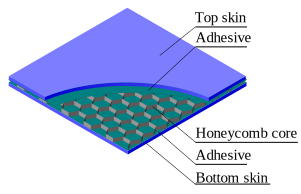
\includegraphics[width=0.95\textwidth]{honeycomb}
	\end{center}
	\caption{Sample configuration: (\textbf{a}) top view of the sample, (\textbf{b}) \acl{hsc} and (\textbf{c}) details of the honeycomb cell}
	\label{fig:honeycomb}
\end{figure*}

The core geometry is accurately reproduced from the actual specimen, i.e., geometry of irregular hexagonal cells \(\left(\mathrm{h}_1 \ne \mathrm{l}_1\right)\) and double walls at the sheet joints, resulting from the core fabrication technology.
According to the drawing in Figure \ref{fig:honeycomb}(\textbf{c}), the cell dimensions are \(\mathrm{w}_c=0.1\) \unit{\mm}, h\(_1\)=11 \unit{\mm}, h\(_2\)=5 \unit{\mm}, l\(_1\)=10.4 \unit{\mm}, l\(_2\)=6 \unit{\mm} and the cell height g=14.5 \unit{\mm}.
The core was bonded to one \ac{cfrp} plate using the epoxy adhesive (Loctite EA3479B) with the thickness h\(_a\)=0.3 \unit{\mm}.
The adhesive layer covered the entire bottom surface of the skin.
Signal excitation and recording were accomplished with a pair of \acp{pzt}  (Noliac, NCE51) mounted to the top surface of the skin with cyanoacrylate glue.
The circular transducers of diameter \(\Phi_{PZT}\)=10 \unit{\mm} and thickness h\(_{PZT}\)=0.5 \unit{\mm} were attached 200 \unit{\mm} apart, as shown in Figure~\ref{fig:honeycomb}(\textbf{a}).
The thickness of cyanoacrylate glue under the \ac{pzt} was assumed to be h\(_g=50\) \unit{\micro\m}.

The material properties of the components assumed for the simulations are compiled in Table~\ref{tab:properties}.
The effective properties of the \ac{cfrp} skin were determined according to the rule of mixtures presented in the book by Vinson and Sierakowski \cite{vinson1993behavior}.
The authors provide a complete description of the homogenisation of composite properties.
Firstly, the stiffness matrix was determined for the single ply of the laminate along the fibre direction.
Then, the stiffness matrix was transformed for other orientations of the laminate plies by the transformation matrix composed of the direction cosines.
In the analysed sample, there were plies with an orientation of \ang{0} and \ang{90}.
Finally, all the plies in the laminate were homogenised through the thickness.
Sun and Li \cite{sun1988three} present the explicit expressions of the stiffness components for the laminate modelled by solid elements.
The comprehensive equations to derive the effective stiffness matrix are given in Appendix~\ref{app:eff_properties}, whereas Table~\ref{tab:properties_eff} shows the resulting \ac{cfrp} properties.
\begin{table*}
	\centering
	\small
	\tabcolsep=0.25cm
	\caption{\label{tab:properties_eff} The homogenised mechanical properties of the \acs{cfrp} plate and the honeycomb core for +20\unit{\degreeCelsius}}
	\begin{tabular}{ccccccccc}
		\toprule
		\multirow{2}{*}{\textbf{Material}} & \(\boldsymbol{E_{11}}\) & \(\boldsymbol{E_{22}}\) & \(\boldsymbol{E_{33}}\) & \(\boldsymbol{G_{12}}\) & \(\boldsymbol{G_{23}}\) & \(\boldsymbol{\nu_{12}}\)	& \(\boldsymbol{\nu_{23}}\) & \(\boldsymbol{\rho}\) \\
		& \unit{\giga\pascal} & \unit{\giga\pascal} & \unit{\giga\pascal} & \unit{\giga\pascal} & \unit{\giga\pascal} & -- & -- & \unit[per-mode = symbol]
		{\kilogram\per\cubic\metre}\\
		\midrule
		\ac{cfrp} & 69.5 & 69.5 & 8.16 & 3.43 & 2.96 & 0.03 & 0.37 & 1555\\
		laminate & & & & & & & &\\
		\midrule
		honeycomb & 0.007 & 0.005 & 2.76 & 0.002 & 0.86 & 0.999 & \(\approx0\) & 112\\
		core & & & & & & & &\\
		\bottomrule
	\end{tabular}
\end{table*}

\subsection{Mesh generation for the \acl{fcgm}}
\label{sec:honeycomb}

%% SECTION CONTENT ////////////////////////////////////////////////////////////////////////////////////
The modelled structure was composed of the following components: 2D for the core, epoxy adhesive and cyanoacrylate glue and 3D for the \ac{cfrp} plate and the \acp{pzt}.
Figure~\ref{fig:struct_mesh} depicts the spectral element used to model the wall, the skin and the \ac{pzt}.
During the creation of the core mesh, special attention was taken to minimise the number of non-zero values in the matrix \(\textbf{G}\).
\begin{figure*}
	\begin{center}
		\includegraphics[width=0.95\textwidth]{struct_mesh}
	\end{center}
	\caption{The mesh with the nodes distribution, (\textbf{a}) spectral element used for modeling the wall of the core, (\textbf{b}) excerpt of the skin plate and (\textbf{c}) cyanoacrylate glue mesh with the second-order curve at the boundary}
	\label{fig:struct_mesh}
\end{figure*}

The core elements were selected for the slave mesh, with one spectral element dedicated to each honeycomb cell wall.
The master meshes of the skin panel and adhesive layer were divided by three rhombic elements into the area under the core cell.
This way, the interface nodes coincided with those on the hexagon edges (red line in Figure~\ref{fig:struct_mesh}(\textbf{b})).
The map of element nodes and their coordinates were generated by custom code developed in Matlab.
The resulting meshes of the core, adhesive layer and skin are shown in Figure \ref{fig:cas_mesh}.

The mesh for the cyanoacrylate adhesive consisted of five elements, with a second-order curve at the structure boundary, as seen in Figure~\ref{fig:struct_mesh}(\textbf{c}).
This structure was connected to the skin with the non-matching interface elements with the adhesive mesh selected as a slave one.
The \ac{pzt} mesh coincided with the glue mesh and they are connected with the matching interface elements.

\begin{figure*}
	\begin{center}
		\includegraphics[width=0.95\textwidth]{cfrp_mesh}
	\end{center}
	\caption{The meshes of \acl{hsc} components and the interfaces between them}
	\label{fig:cas_mesh}
\end{figure*}

%% SECTION HEADER /////////////////////////////////////////////////////////////////////////////////////
\subsection{\Acl{hcgm}}
\label{sec:homogenised}

%% SECTION CONTENT ////////////////////////////////////////////////////////////////////////////////////
Section \ref{sec:modelling} contains several examples of the successful application of the model to numerical analysis of \ac{gw} propagation and damage localisation in \ac{hsc}.
Its unquestionable advantage is the simplified component mesh, reducing operating memory resources.
In the dissertation, comparative studies between the \ac{hcgm} and the \ac{fcgm} were conducted to assess the simplified model effectiveness in estimating damage size.

In the \ac{hcgm}, the values of the material constants of the panel core were calculated according to the method presented by Malek and Gibson \cite{malek2015effective}.
This model is an extension of the theoretical analysis of Gibson et al. \cite{gibson1982mechanics}, considering the different geometry of the cell and the nodes at the intersection of the vertical and inclined walls.

The comprehensive formulation of the stiffness matrix components is given in Appendix~\ref{app:eff_properties} and the effective mechanical properties are gathered in Table \ref{tab:properties_eff}.
The properties for other structures, i.e., the skin, the epoxy adhesive, the cyanoacrylate glue, and the sensors remained unchanged.
The core element has \(6 \times 6 \times 4\) nodes, and the mesh coincides with the skin mesh.
The elements of the other structures are the same as described in the previously.

%% SECTION HEADER /////////////////////////////////////////////////////////////////////////////////////
\subsection{Damaged structure implementation}
\label{sec:disbond}
%% SECTION CONTENT ////////////////////////////////////////////////////////////////////////////////////
The skin and the core disbonds were evaluated to analyse the effect of damage on GW propagation.
A rectangular region of disbonds was investigated with the length along the wave propagation varying in width \(\mathrm{w_d} = [0,10,30,50,70,100,120]\) mm, and the damage length in the perpendicular direction was constant \(\mathrm{l_d} = 170\) mm.
The rectangle was centrally located between the transducers, as presented in Figure~\ref{fig:honeycomb}(\textbf{a}).
The selected dimensions of the defects correspond to the dimensions of disbonds made in the specimen to be measured experimentally.
The damage was done with a sharp hooked tool that detached the core from the adhesive layer cell by cell.
The dimensions of the disbond had a coarse tolerance, measuring the width by a calliper.
Due to the small aluminium sheet thickness, the core cells were squashed within the damaged area as it can be seen in Figure~\ref{fig:disbond}\textbf{(a)}.

Two kinds of disbond models were considered in the analysis.
The core cells were removed from the damaged area in the first model as in the mesh pictured in Figure~\ref{fig:disbond}(\textbf{b}).
Whereas in the second model, all components were intact, and only the interface elements between the adhesive layer and the core were decoupled within the yellow area indicated in Figure~\ref{fig:disbond}(\textbf{c}).
\begin{figure*}[!bh]
	\begin{center}
		\includegraphics[width=0.9\textwidth]{disbond}
	\end{center}
	\caption{The damaged area in the: (\textbf{a}) experimental sample,(\textbf{b}) numerical model with removed cells and (\textbf{c}) numerical model with interface decoupling}
	\label{fig:disbond}
\end{figure*}

\section{The Severity of Damage Estimation}
\subsection{Damage indices}
\label{sec:di}

%% SECTION CONTENT ////////////////////////////////////////////////////////////////////////////////////
In the dissertation, six damage indices, considered to be the most effective \cite{torkamani2014novel, moix2016damage}, were analysed based on the signal envelope in the time-domain registered by the sensor.
All of them were considered in three variants: (i) the full-length of the signal, (ii) the first wave packet of the \ac{s0}, (iii) the first wave packet of the \ac{a0}.
The analysis considered signals at 50, 100 and 150 \unit{\kHz}, with the last frequency excluded for the \ac{a0}, because, as indicated in Section~\ref{sec:resuls_pzt}, this mode was masked by reflections of the \ac{s0}.
The wave packets were extracted by windowing the full-length signals with a flattened Gaussian window in the form
\begin{eqnarray}
	g(t)= \mathrm{exp}\left(-\left(\frac{t-t_0}{w_g}\right) ^{s}\right),
	\label{eq:psi_g}
\end{eqnarray}
where \(t_0\) and \(w_g=0.5N_c/f_c\) are the center point and the half-width of the window, respectively, and \(s\) determines the slope of the window. Figure~\ref{fig:windows} depicts the usage of the window.
\begin{figure*}[!tbh]
	\begin{center}
		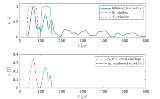
\includegraphics[width=0.95\textwidth]{windows}
	\end{center}
	\caption{The signal envelop and the Gaussian windows}
	\label{fig:windows}
\end{figure*}

The following time-domain indices were taken into consideration: \ac{p2p}, \ac{saps}, \ac{sapr}, \acf{rmsd}, \ac{eng} and \ac{cc}.
Definitions of these metrics are as follows:
\begin{eqnarray}
	\mathrm{P2P} = \mathrm{max}(e_H) - \mathrm{max}(e_D),\\
	\mathrm{SAPS} = 1 - \left[\frac{\mathrm{max}(e_H)-\mathrm{max}(e_D)}{\mathrm{max}(e_H)}\right]^2,\\
	\mathrm{SAPR} = \frac{\mathrm{max}(e_H)}{\mathrm{max}(e_D)},\\
	\mathrm{RMSD} = 1 - \sqrt{\frac{\sum_{i=1}^{l}\left(e_D-e_H\right)^2}	{\sum_{i=1}^{l}e_H^2}},\\
	\mathrm{ENG} = 1 -  \frac{\sum_{i=1}^{l}{e_D^2}-\sum_{i=1}^{l}{e_H^2}}{\sum_{i=1}^{l}{e_H^2}},
\end{eqnarray}

\begin{multicols}{1}
\begin{equation}
	\begin{split}	
	\mathrm{CC}  = \frac{l\sum_{i=1}^{l}e_De_H-\sum_{i=1}^{l}e_D\sum_{i=1}^{l}e_H}{\sqrt{l\sum_{i=1}^{l}e_D^2-\left[\sum_{i=1}^{l}e_D\right]^2}\sqrt{l\sum_{i=1}^{l}e_H^2-\left[\sum_{i=1}^{l}e_H\right]^2}},
	\end{split}
\end{equation}
\end{multicols}
where \(e_H\) and \(e_D\) are the envelope of the signal registered by the sensor for the healthy and damaged state of the specimen, respectively, \(l\) is the length of the signal, and max\((e)\) is maximum value of the signal envelope.
The \ac{p2p}, \ac{saps}, \ac{sapr} are based on the difference between amplitudes of the monitored and the baseline state.
The \ac{rmsd} measures the error between baseline and damaged, \ac{eng} compares the difference of the sensor responses energy and \ac{cc} is the index based on Pearson correlation coefficient.

\begin{figure*}[!tbh]
	\begin{center}
		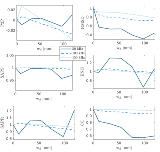
\includegraphics[width=0.95\textwidth]{DI_full_full}
	\end{center}
	\caption{The \aclp{di} obtained with the \acl{fcgm} based on the full-length signals}
	\label{fig:DI_full_full}
\end{figure*}

\begin{figure*}[!tbh]
	\begin{center}
		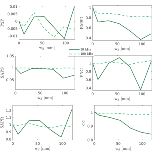
\includegraphics[width=0.95\textwidth]{DI_full_A0}
	\end{center}
	\caption{The \aclp{di} obtained with the \acl{fcgm} based on the \acs{a0} windowed signal}
	\label{fig:DI_full_A0}
\end{figure*}

\begin{figure*}[!tbh]
	\begin{center}
		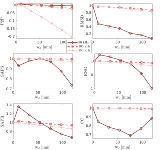
\includegraphics[width=0.95\textwidth]{DI_full_S0}
	\end{center}
	\caption{The \aclp{di} obtained with the \acl{fcgm} based on the \acs{s0} windowed signal}
	\label{fig:DI_full_S0}
\end{figure*}

The \acp{di} based on full-length signals derived from simulations with the \ac{fcgm} are presented in Figure~\ref{fig:DI_full_full}.
The damage was modelled by removing the core cells in the damage area.
Noticeably, all the \acp{di} for 50 \unit{\kHz} are not monotonous.
This is due to the fact that a low-frequency wave (up to 100 \unit{\kHz}, according to work of Tian et al. \cite{tian2015wavenumber}), propagated through the entire thickness of \ac{hsc}.
Therefore, in the analysis of damage size, not only the phenomenon of wave leakage was relevant, but also the reflection from cell walls.  
The high-frequency wave propagated mainly through the skin of the panel, so changes in the signal recorded by the sensor in the damaged sample were mainly caused by the wave leakage effect.

The \acp{di} based on the windowed signals are shown in Figures~\ref{fig:DI_full_A0} and \ref{fig:DI_full_S0} for the \ac{a0} and \ac{s0} window, respectively.
It should be mentioned that \acp{di} for 150 \unit{\kHz} were omitted in Figure~\ref{fig:DI_full_A0}, due to the masking of this mode by the \ac{s0} reflections.
The characteristics of the \ac{s0}-based indices are consistent with the related indices determined for the full-length signals, although for most indices, their values are less than those of full-length signals.
The \ac{s0}-based \acp{di} values are also less than the \ac{a0}-based signals, except the \ac{rmsd} at 50 \unit{kHz}.
It is because dominant displacements of the \ac{s0} are in-plane of the skin, so less portion of the wave energy leak into the core through the healthy region.
In the case of the full-length response, the \ac{a0} was registered, which is more susceptible to damage in the form of disbonds or delamination since its main displacements are out-of-plane.

Accordingly, the following indicators were selected for further consideration: \ac{p2p} and \ac{sapr} at 150 \unit{kHz} (see Figures \ref{fig:DI_P2P} and \ref{fig:DI_SAPR}), \ac{rmsd} and \ac{cc}, all in the case of full-length and at 100 and 150 \unit{\kHz} (see Figures \ref{fig:DI_RMSD_full} and \ref{fig:DI_CC}), and \ac{rmsd} at 50 \unit{kHz} \ac{s0}-based signals (see Figure \ref{fig:DI_RMSD_S0}).
Selected indicators were also determined for damage modeled by removing interface elements. Then, they were compered with the indices obtained for the \ac{hcgm}.

\begin{figure}
	\begin{center}
		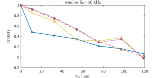
\includegraphics{DI_P2P}
	\end{center}
	\caption{Comparison of the selected \acfp{p2p} based on full-length signals for the various models of the core and damage: the \acf{fcgm} with removed core cells (solid line), the \ac{fcgm} with removed interface elements (dashed line), the \acf{hcgm} with removed core cells (dash-dot line), the \ac{hcgm} with removed interface elements(dotted line)}
	\label{fig:DI_P2P}
\end{figure}

\begin{figure*}[!tbh]
	\begin{center}
		\includegraphics[width=0.95\textwidth]{DI_SAPR}
	\end{center}
	\caption{Comparison of the selected \acfp{sapr} based on full-length signals for the various models of the core and damage: the \acf{fcgm} with removed core cells (solid line), the \ac{fcgm} with removed interface elements (dashed line), the \acf{hcgm} with removed core cells (dash-dot line), the \ac{hcgm} with removed interface elements (dotted line)}
	\label{fig:DI_SAPR}
\end{figure*}
It can be noticed that \ac{p2p} and \ac{sapr} differ significantly in terms of the core model used. Both indexes for the \ac{fcgm} are continuously decreasing, while for the \ac{hcgm}, the values are almost constant in the whole range of damage.
In addition, the damage model has little effect only for the \ac{fcgm}.
The values for all cases are consistent for the \ac{rmsd} based on the \ac{s0} window.
Only the \ac{fcgm} for the two smallest damage scenarios deviates from the other models.
For the \ac{rmsd} and the \ac{cc} based on full-length signals, the results are comparable for the all models, except the values for the \ac{hcgm} at 100 \unit{kHz} are more significant than the \ac{fcgm}.
\begin{figure*}[!tbh]
	\begin{center}
		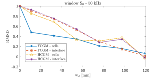
\includegraphics[width=0.95\textwidth]{DI_RMSD_S0}
	\end{center}
	\caption{Comparison of the selected \acfp{rmsd} based on \ac{s0} windowed signals for the various models of the core and damage: the \acf{fcgm} with removed core cells (solid line), the \ac{fcgm} with removed interface elements (dashed line), the \acf{hcgm} with removed core cells (dash-dot line), the \ac{hcgm} with removed interface elements (dotted line)}
	\label{fig:DI_RMSD_S0}
\end{figure*}

\begin{figure*}[!tbh]
	\begin{center}
		\includegraphics[width=0.95\textwidth]{DI_RMSD_full}
	\end{center}
	\caption{Comparison of the selected \acfp{rmsd} based on full-length signals for the various models of the core and damage: the \acf{fcgm} with removed core cells (solid line), the \ac{fcgm} with removed interface elements (dashed line), the \acf{hcgm} with removed core cells (dash-dot line), the \ac{hcgm} with removed interface elements (dotted line)}
	\label{fig:DI_RMSD_full}
\end{figure*}

\begin{figure*}[!bh]
	\begin{center}
		\includegraphics[width=0.95\textwidth]{DI_CC_full}
	\end{center}
	\caption{Comparison of the selected \acfp{cc} based on full-length signals for the various models of the core and damage: the \acf{fcgm} with removed core cells (solid line), the \ac{fcgm} with removed interface elements (dashed line), line the \acf{hcgm} with removed core cells (dash-dot), the \ac{hcgm} with removed interface elements (dotted line)}
	\label{fig:DI_CC}
\end{figure*}

%% Loading bibliography style file
%\bibliographystyle{model1-num-names}
\bibliographystyle{cas-model2-names}

% Loading bibliography database
\bibliography{model_hc}

\end{document}

